\documentclass{article}
\usepackage[swedish]{babel}
\usepackage[utf8]{inputenc}
\usepackage{amsmath} 

\usepackage{fancyhdr}
\usepackage{lastpage}
\usepackage{lineno}
\usepackage{lmodern}
\usepackage[T1]{fontenc}
\usepackage[utf8]{inputenc}
\usepackage[swedish]{babel}
\usepackage{microtype}
\usepackage{systeme}
\usepackage{amsmath,amssymb,amsthm,mathrsfs,latexsym,tikz,url}
\usepackage{epigraph,graphicx}
%\usepackage{titlesec} %For formatting sections
\usepackage{listings}
\usepackage{listingsutf8}
\usepackage{color}
\usepackage{todonotes}
\presetkeys%
    {todonotes}%
    {inline,backgroundcolor=yellow}{}

\graphicspath{ {./}{./figures/} {images/}}
\DeclareGraphicsExtensions{.png,.pdf}

\definecolor{dkgreen}{rgb}{0,0.6,0}
\definecolor{gray}{rgb}{0.5,0.5,0.5}
\definecolor{mauve}{rgb}{0.58,0,0.82}

\lstset{frame=tb,
  language=Python,
  aboveskip=3mm,
  belowskip=3mm,
  showstringspaces=false,
  columns=flexible,
  basicstyle={\small\ttfamily},
  numbers=none,
  numberstyle=\tiny\color{gray},
  keywordstyle=\color{blue},
  commentstyle=\color{dkgreen},
  stringstyle=\color{mauve},
  breaklines=true,
  breakatwhitespace=true,
  tabsize=4
}


\setlength{\parindent}{0.0cm}
\setlength{\parskip}{0.1cm}



\begin{document}


\title{Lab 1 Machine Learning}
\author{Anton Stråhle \& Jan Alexandersson}
\maketitle 

\section*{Dual formulation}

The minimization of the objective can be written as

\begin{align*}
\min_{\alpha_1,...,\alpha_n} \frac{1}{2}
 \begin{bmatrix}
\alpha_1 \\
\alpha_2 \\
\vdots \\
\alpha_n 
\end{bmatrix}^{T}
 \begin{bmatrix}
t_1 t_1 \kappa (\vec{x}_1, \vec{x}_2) & \hdots & t_1 t_n \kappa (\vec{x}_1, \vec{x}_n) \\
\vdots & \ddots & \\
t_n t_1 \kappa (\vec{x}_n, \vec{x}_1) &  & t_n t_n \kappa (\vec{x}_n, \vec{x}_n)
\end{bmatrix}
\begin{bmatrix}
\alpha_1 \\
\alpha_2 \\
\vdots \\
\alpha_n 
\end{bmatrix}
+
\begin{bmatrix}
-1 \\
\vdots \\
-1 
\end{bmatrix}^{T}
\begin{bmatrix}
\alpha_1 \\
\alpha_2 \\
\vdots \\
\alpha_n 
\end{bmatrix}
\end{align*}

with the corresponding constraints

\begin{align*}
\begin{bmatrix}
-1 & \hdots & 0 \\
\vdots & \ddots & \\
0  &  & -1 \\
1 & \hdots & 0 \\
\vdots & \ddots & \\
0  &  & 1
\end{bmatrix}
 \begin{bmatrix}
\alpha_1 \\
\alpha_2 \\
\vdots \\
\alpha_n 
\end{bmatrix}
\preccurlyeq
 \begin{bmatrix}
0 \\
\vdots \\
0 \\
C \\
\vdots \\
C
\end{bmatrix}.
\end{align*}


We solve this using the QP function in the CVXOPT package. 

\section*{Assignment 1}

\begin{itemize}
 \item An optimal solution can not be found using a linear kernel if the classes are not lineary separable.
 \item An optimal solution can not be found if the data is not separable with the polynomial degree used. 
 For example, degree 3 may work but degree 2 may not, then data is separable with the degree 3. 
 \item When using a radial kernel, an optimal solution can not be found if the data is not separable at all. 
\end{itemize}

\section*{Assignment 2}

\begin{lstlisting}
def radial_kernel(x, y):
    diff = np.subtract(x, y)
    return math.exp((-np.dot(diff, diff)) / (2 * SIGMA * SIGMA))

def polynomial_kernel(x, y):
	return np.power((np.dot(x, y) + 1), POLYNOMIAL_GRADE)
\end{lstlisting}

\section*{Assignment 3}

When using a polynomial kernel a higher degree or will classify more precise accordiong to the training set which will increase 
the variance but decreasing the bias. 
Similarily, when using a Radial Basis Function kernel a lower sigma will increase variance and decrease bias. 
This may lead to overfitting. 

\section*{Assignment 4}

If C is small, then there will be fewer support vectors and hence the resulting classifier will have low bias but
high variance. This is because a low value of C does not allow for the margins to be as violated as a high value. 

\section*{Assignment 5}

If we have a noicy dataset, i.e. multiple points deviating from the main clusters we should not opt for a more complex kernel since this would in some sense overfit the boundary to include these specific outliers which of course would impact future predictions negativeley. Instead we should allow for extra slack by increasing $C$, thus sacrificing some predictive power by obtaining a more general, and hopefully better predicting, boundary. 

If we however have have a very sparse and spread out data with no clear major clusters we should consider using a more complex model to be able to incorporate the spread of the different classes. By allowing for extra slack in this case we might obtain a boundry that missclassifies certain minor classes which of course is not to be desired. In these cases with a lot of spread and no clear clusters we might also question the use of SVM entierly.

\section*{Appendix}

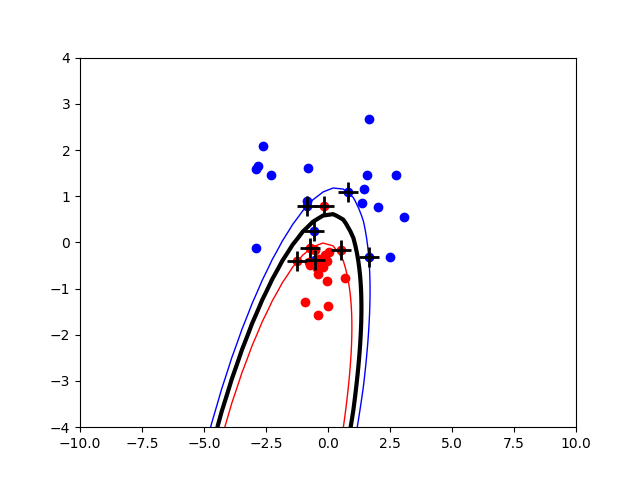
\includegraphics[scale = 0.66]{Figure_1.png}

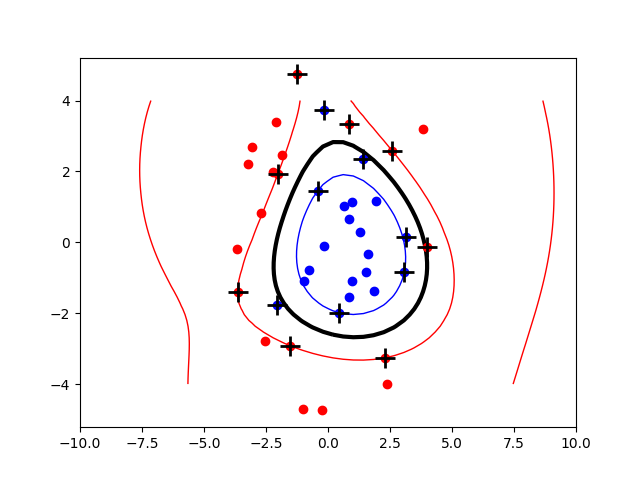
\includegraphics[scale = 0.66]{Figure_2.png}

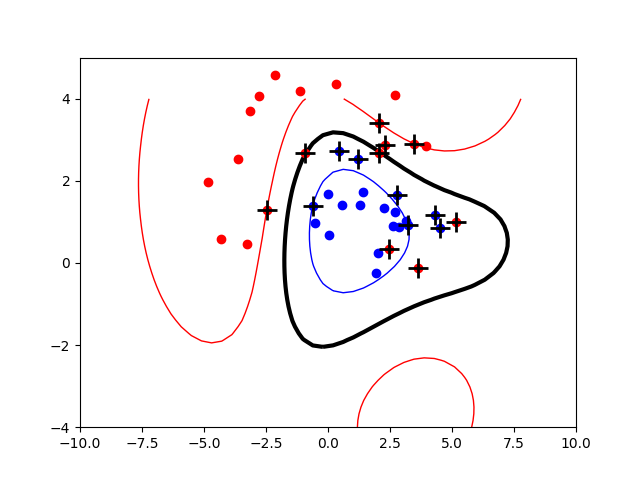
\includegraphics[scale = 0.66]{Figure_3.png}

\end{document}
